\subsection{Hardware}

Las pruebas de Hardware permiten conocer el funcionamiento real de los componentes de un sistema bajo ciertas condiciones las cuáles, pretenden simular el entorno al que el sistema será expuesto cuando éste entre en funcionamiento.

Dentro de este Trabajo Teminal, existen tres componentes que integran todo el hardware de nuestro sistema: El caudalimetro, el microcontrolador y el sensor Bluetooth loc cuáles estan intercoectados entre sí de manera física, a través de una conexión cableada.

Dichos componentes estarán en contacto con las bombas dispensadoras de gasolina que a través de las pistolas se encargan de ingresar la gasolina al vehículo. 

\paragraph{Creación nuestro ambiente de pruebas}
El ambiente ideal para poder probar nuestro sistema es dentro de una gasolinera, en la cuál podamos poner nuestro circuito electrónico en la entrada del tanque de combustible y conectar las pistolas de los dispensadores de gasolina a nuestro circuito.
De esta forma, la gasolina fluirá desde el dispensador hasta nuestro automóvil pasando a través de nuestro sensor.

A continuación se muestra una imagen que describe el proceso antes mencionado.

\begin{figure}[H]
	\centering
	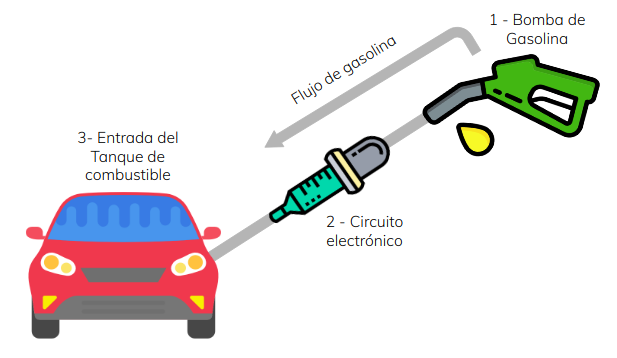
\includegraphics[scale=.60]{DocumentoTecnico/Capitulo6/images/flujo_uno}
	\caption{Descripción de la colocación del sensor}
	\label{fig:flujo_uno}
\end{figure}

A continuación se muestras las pruebas unitarias correspondientes a cada uno de los submódulos del hardware.

\section{Pruebas de integración}
A continuación se muestran las pruebas de integración de los módulos de hardware y software.
\section{Pruebas de integración}
A continuación se muestran las pruebas de integración de los módulos de hardware y software.
\input{Capitulo6/integracion//Hardware/principal}
\input{Capitulo6/integracion//Software/principal}


\section{Pruebas de integración}
A continuación se muestran las pruebas de integración de los módulos de hardware y software.
\input{Capitulo6/integracion//Hardware/principal}
\input{Capitulo6/integracion//Software/principal}




\section{Pruebas de integración}
A continuación se muestran las pruebas de integración de los módulos de hardware y software.
\section{Pruebas de integración}
A continuación se muestran las pruebas de integración de los módulos de hardware y software.
\input{Capitulo6/integracion//Hardware/principal}
\input{Capitulo6/integracion//Software/principal}


\section{Pruebas de integración}
A continuación se muestran las pruebas de integración de los módulos de hardware y software.
\input{Capitulo6/integracion//Hardware/principal}
\input{Capitulo6/integracion//Software/principal}







